\appendix
\pagenumbering{roman}% resets `page` counter to 1
\section*{Appendix}

% New Figure Counter for Appendix with A. prefix
\counterwithin*{figure}{part}
\stepcounter{part}
\renewcommand{\thefigure}{A.\arabic{figure}}

\FloatBarrier
\subsection*{GAN Inversion}
\begin{figure}[!ht]
    \centering
    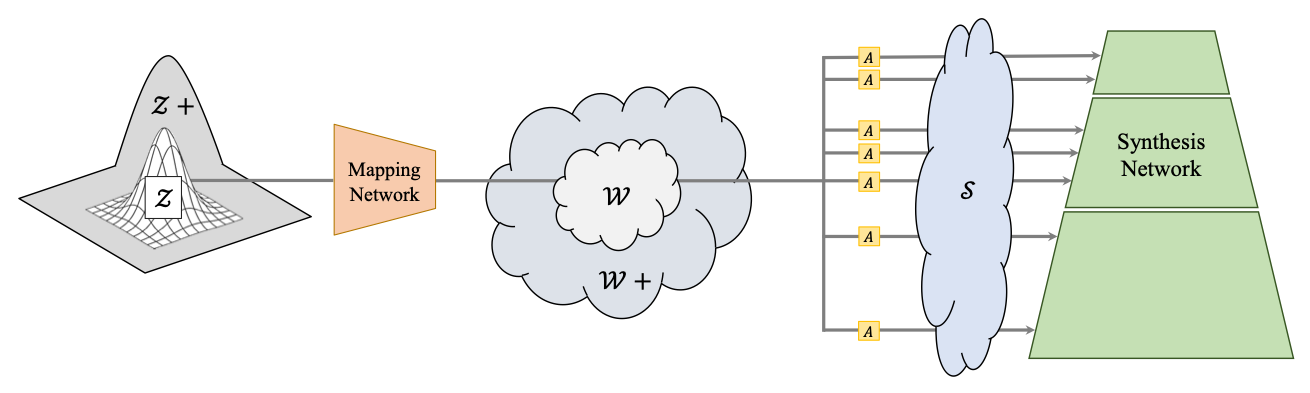
\includegraphics[width=1\linewidth]{Thesis/Background/assets/latent_spaces.png}
    \caption[StyleGAN Latent Spaces]{StyleGAN Latent Spaces - taken from \cite{bermano2022state}}
    \label{fig:latent_spaces}
\end{figure}

\begin{figure}[!ht]
    \centering
    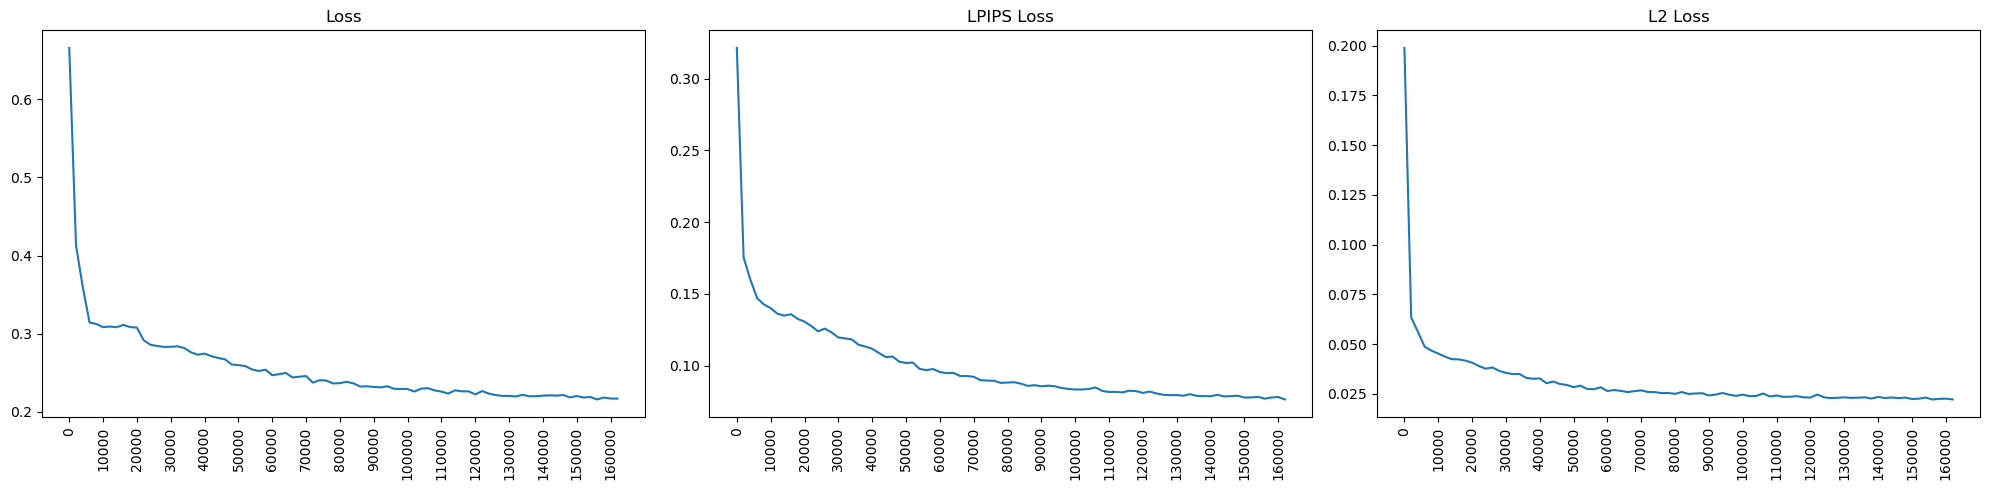
\includegraphics[width=1\linewidth]{Thesis/Method/assets/e4e_loss_curves.png}
    \caption{encoder4editing Training Loss Curves}
    \label{fig:e4e_loss_curves}
\end{figure}

\begin{figure}[!ht]
     \centering
     \begin{subfigure}[b]{1\textwidth}
         \centering
         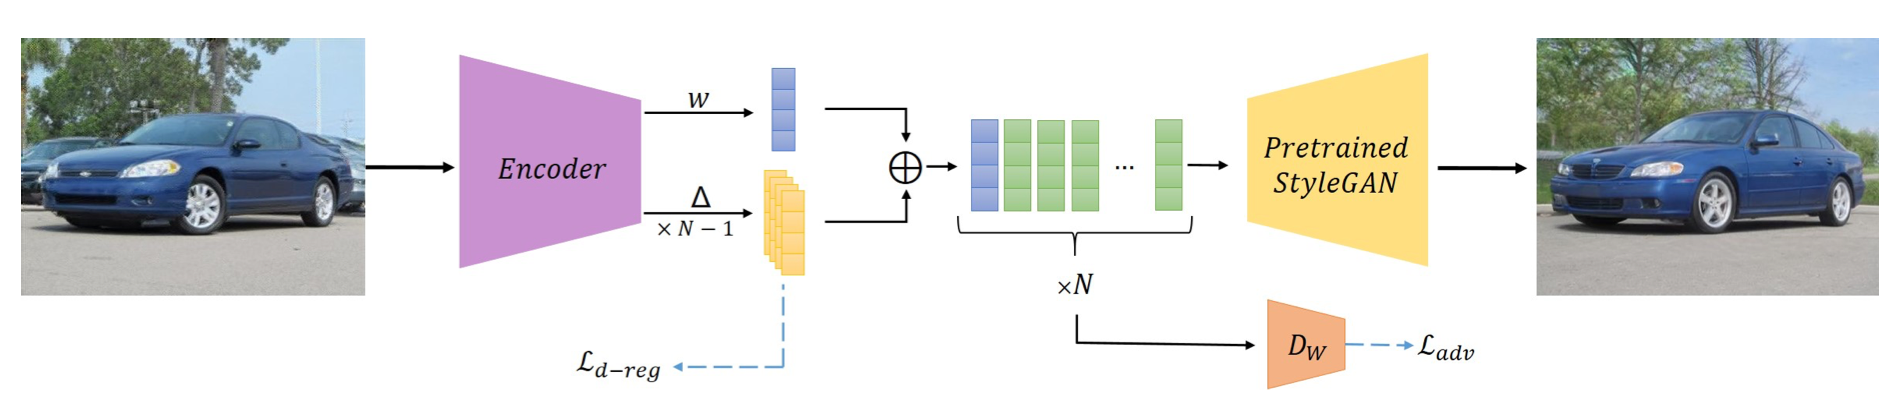
\includegraphics[width=0.95\linewidth]{Thesis/Background/assets/e4e.png}
         \caption{encoder4editing - taken from \cite{tov2021designing}}
         \label{fig:e4e}
     \end{subfigure}
     \hfill
     \begin{subfigure}[b]{1\textwidth}
         \centering
         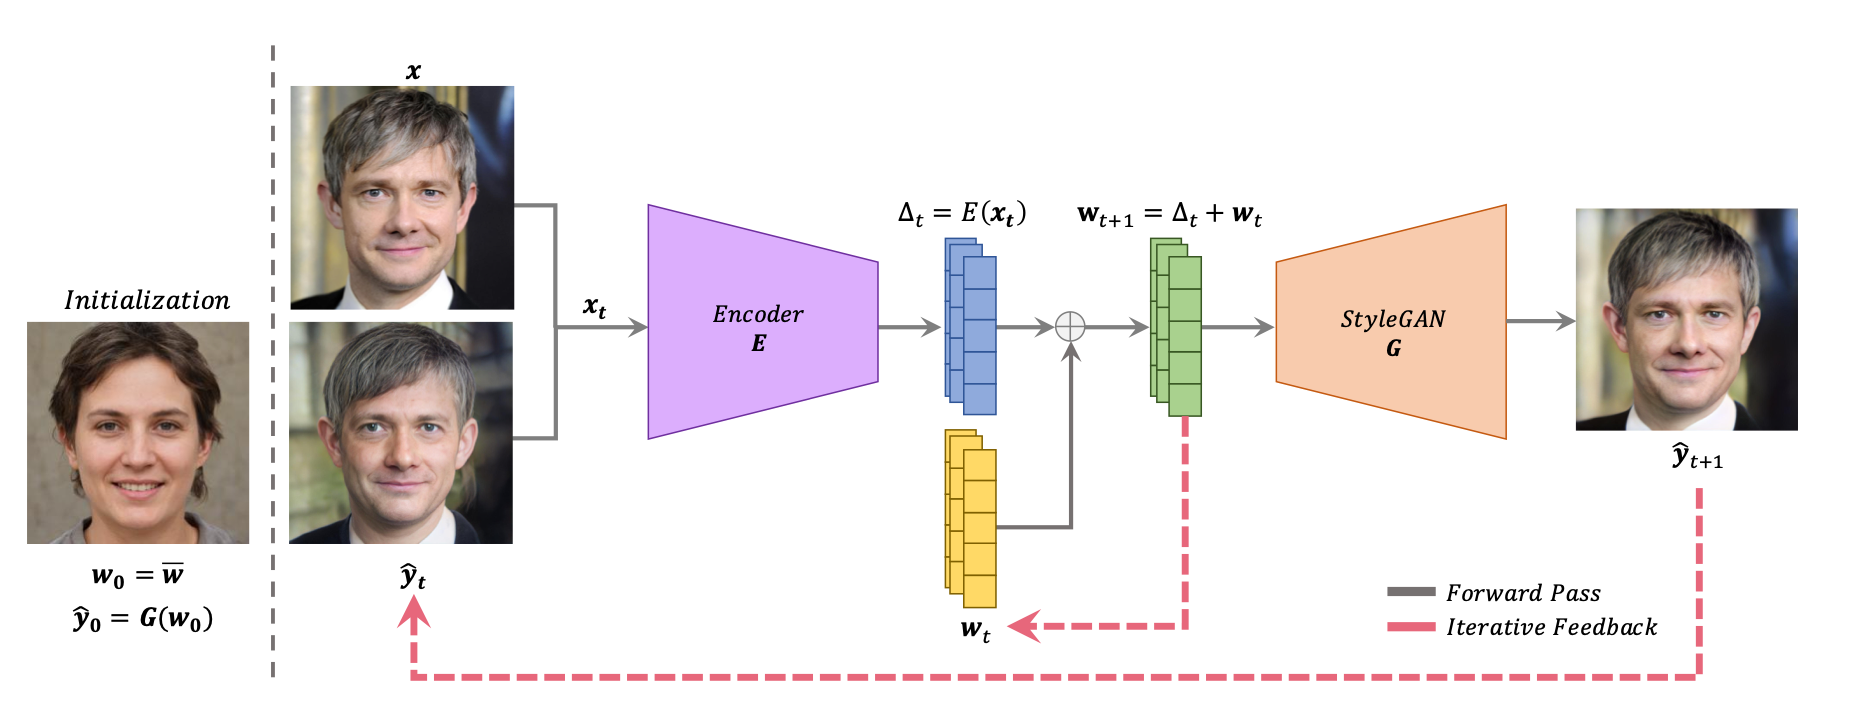
\includegraphics[width=0.95\linewidth]{Thesis/Background/assets/restyle.png}
         \caption{ReStyle - taken from \cite{alaluf2021restyle}}
         \label{fig:restyle}
     \end{subfigure}
     \hfill
     \begin{subfigure}[b]{1\textwidth}
         \centering
         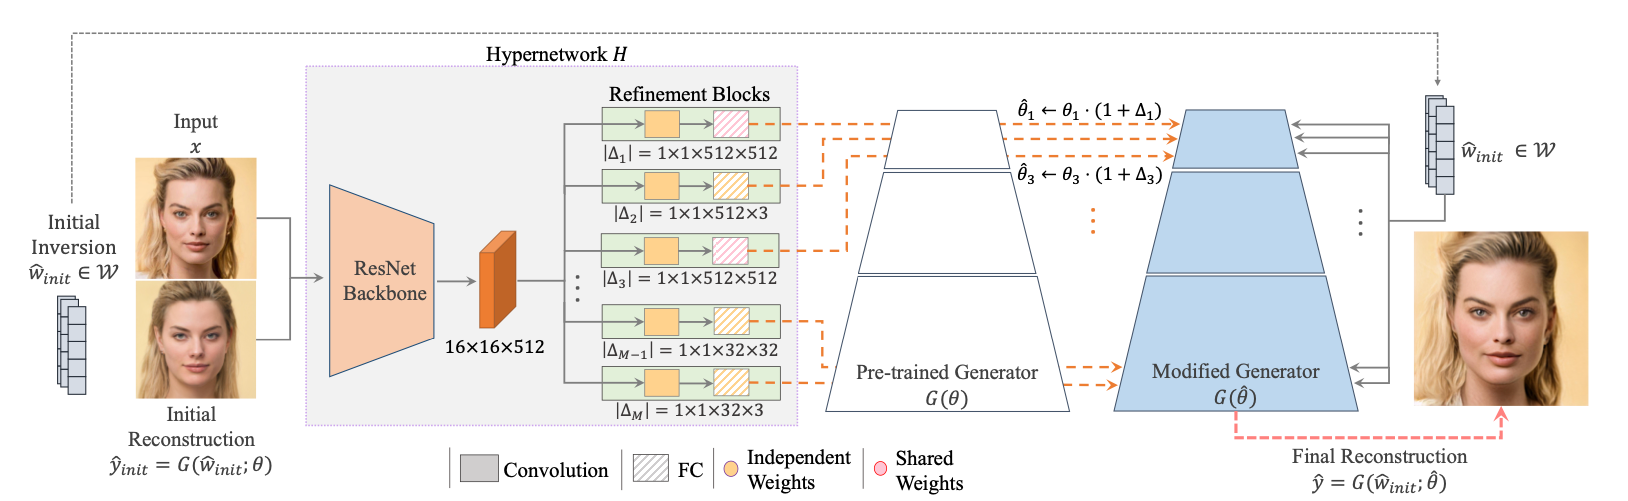
\includegraphics[width=0.95\linewidth]{Thesis/Background/assets/hyperstyle.png}
         \caption{HyperStyle - taken from \cite{alaluf2022hyperstyle}}
         \label{fig:hyperstyle}
     \end{subfigure}
        \caption{Schematic Overview of Inversion Methods}
        \label{fig:inversion_methods}
\end{figure}

\FloatBarrier
\clearpage
\subsection*{StyleGAN2-Ada Training}
\begin{figure}[ht!]
    \centering
    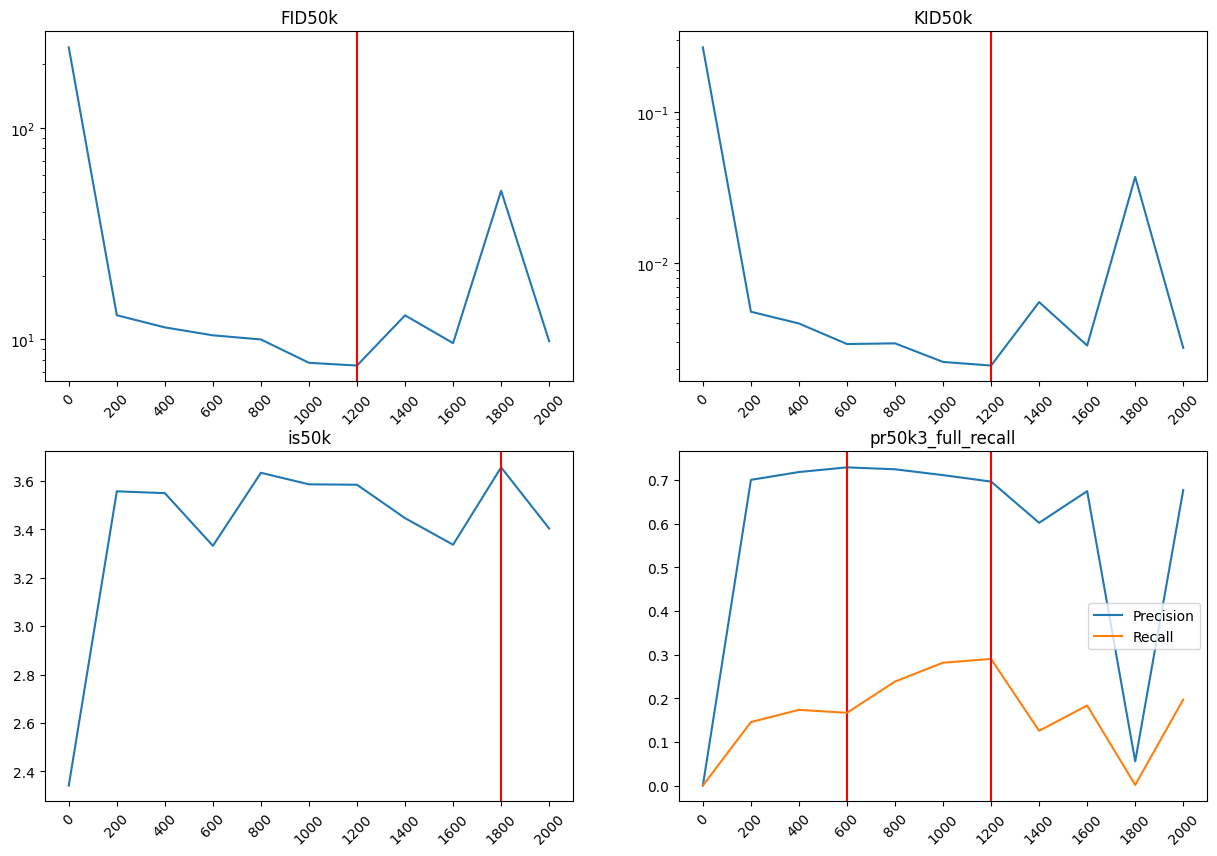
\includegraphics[width=1\linewidth]{Thesis/Results/assets/sg2ada_evaluation_metrics.png}
    \caption[StyleGAN2-Ada Training Evaluation]{StyleGAN2-Ada Training Evaluation: \textit{Red lines indicate best values within each metric. FID50k, KID50k, and IS50k refer to the FID, KID, and IS calculated based on 50k generated images.}}
    \label{fig:sg2ada_evaluation_metrics}
\end{figure}

\FloatBarrier
\clearpage
\subsection*{InterFaceGAN}
\begin{figure}[!ht]
    \centering
    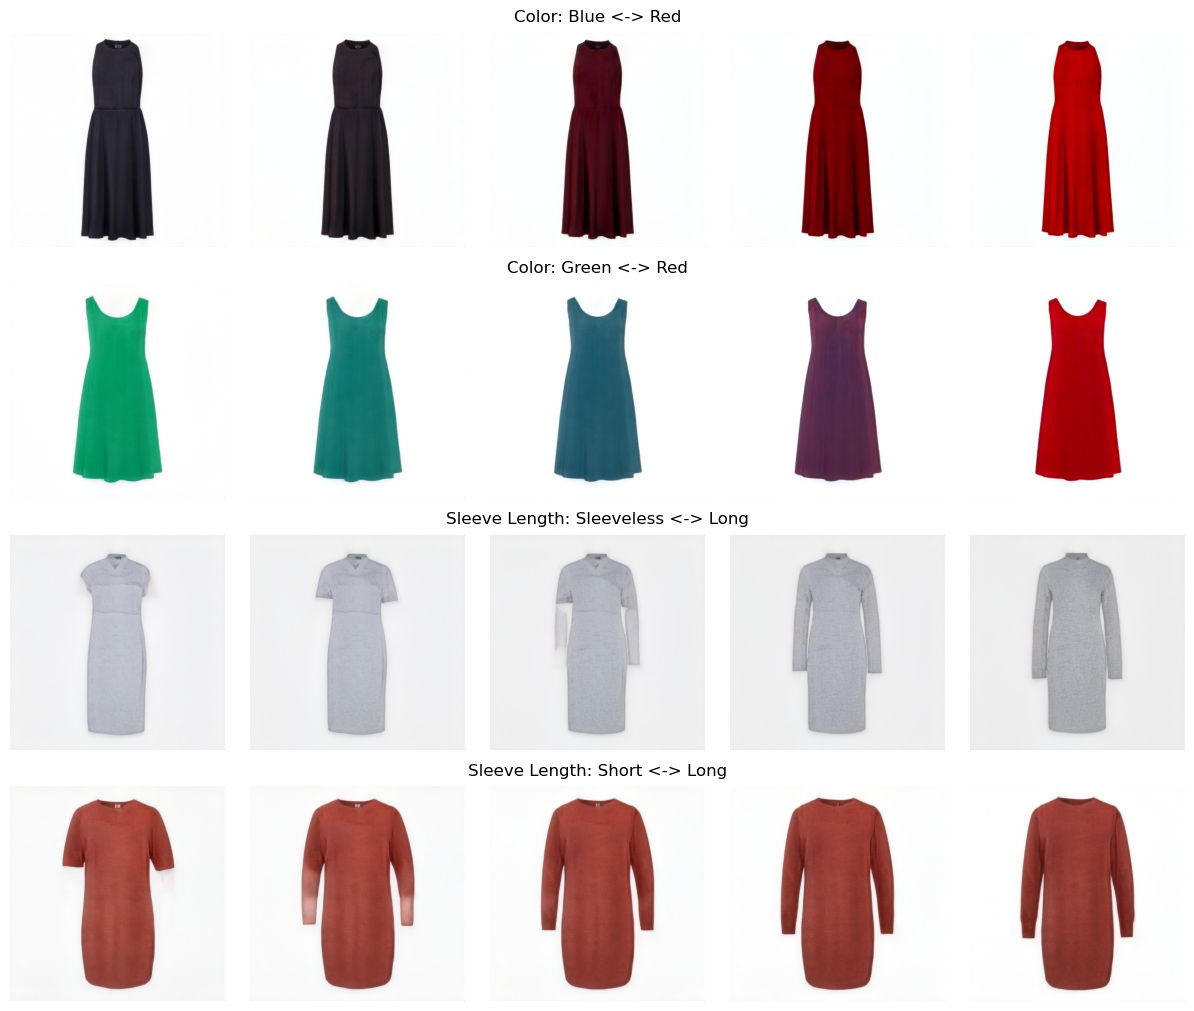
\includegraphics[width=1\linewidth]{Thesis/Method/assets/physical_attributes_manipulation.png}
    \caption[Manipulations of Physical Attributes Used as Conditions]{Manipulations of physical attributes used as conditions: \textit{Physical attributes are used as conditional boundaries for the typicality manipulation. To visually validate that the boundaries are meaningful, one can look at manipulations using the boundaries. All images are generated from e4e inversions.}}
    \label{fig:physical_attributes_manipulation}
\end{figure}


\begin{table}[ht]
\centering
\begin{tabular}{|c|c|c|}
\hline
       &      Color &   Sleeve Length \\
\hline
 count & 91      &         54      \\
 mean  &  0.9595 &          0.9673 \\
 std   &  0.0324 &          0.0506 \\
 min   &  0.8736 &          0.7647 \\
 25\%   &  0.9359 &          0.965  \\
 50\%   &  0.9694 &          0.9885 \\
 75\%   &  0.9859 &          0.9962 \\
 max   &  1      &          1      \\
\hline
\end{tabular}
\caption{Summary Statistics of Separation Performance for Physical Attributes}
\label{tab:physical_summary_stats}
\end{table}

\FloatBarrier
\subsection*{Typicality Measurements}
\begin{figure}[!ht]
    \centering
    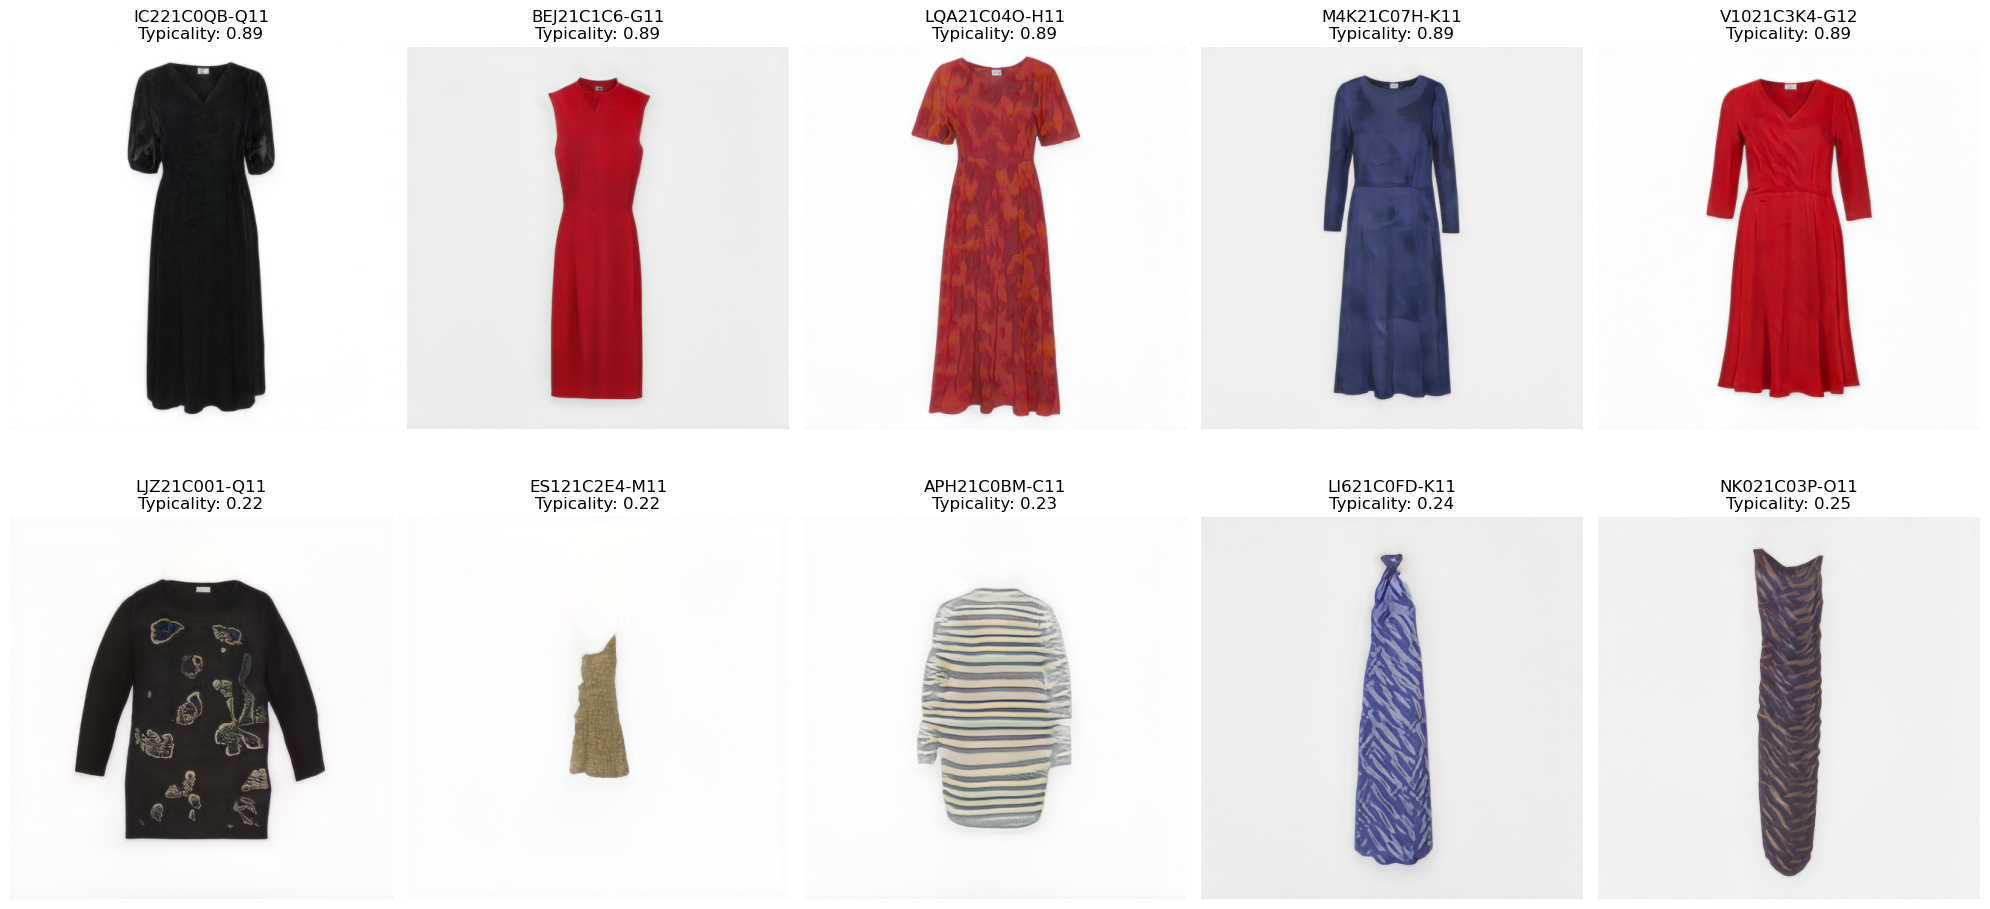
\includegraphics[width=1\linewidth]{Thesis/Results/assets/examples_dino_typicality.png}
    \caption[Most and Least Typical Dresses based on DINOv2 Embeddings]{Most and Least Typical Dresses based on DINOv2 Embeddings: \textit{Top row shows samples with the highest typicality scores, bottom row shows samples with the lowest typicality scores}}
    \label{fig:examples_dino_typicality}
\end{figure}

\begin{figure}[!ht]
    \centering
    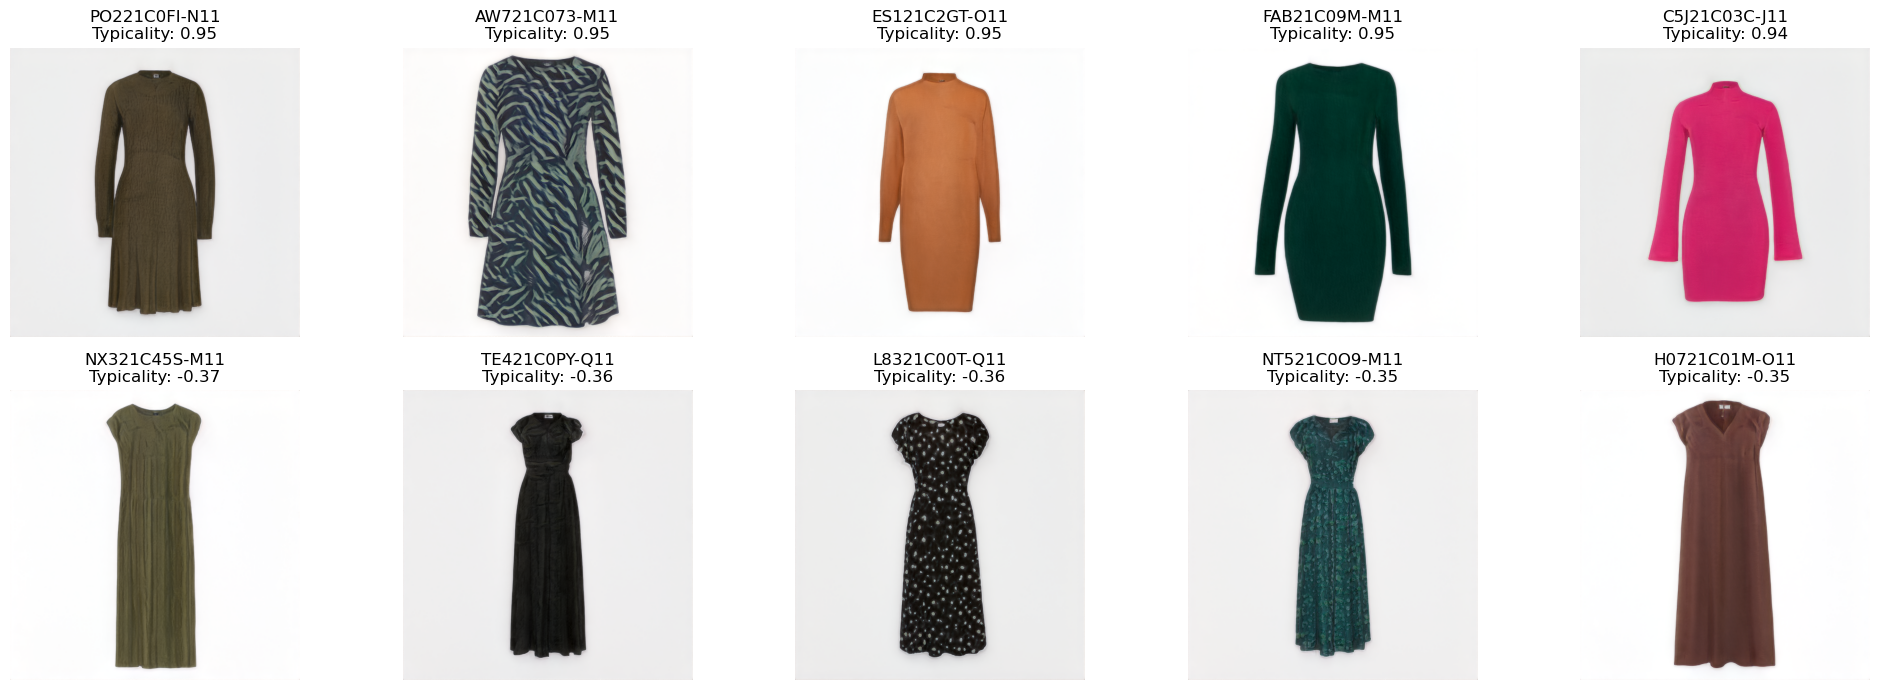
\includegraphics[width=1\linewidth]{Thesis/Results/assets/examples_disentangled_typicality.png}
    \caption[Most and Least Typical Dresses based on Complete Disentangled Embeddings]{Most and Least Typical Dresses based on Complete Disentangled Embeddings: \textit{Top row shows samples with the highest typicality scores, bottom row shows samples with the lowest typicality scores}}
    \label{fig:examples_disentangled_typicality}
\end{figure}

\begin{figure}[!ht]
    \centering
    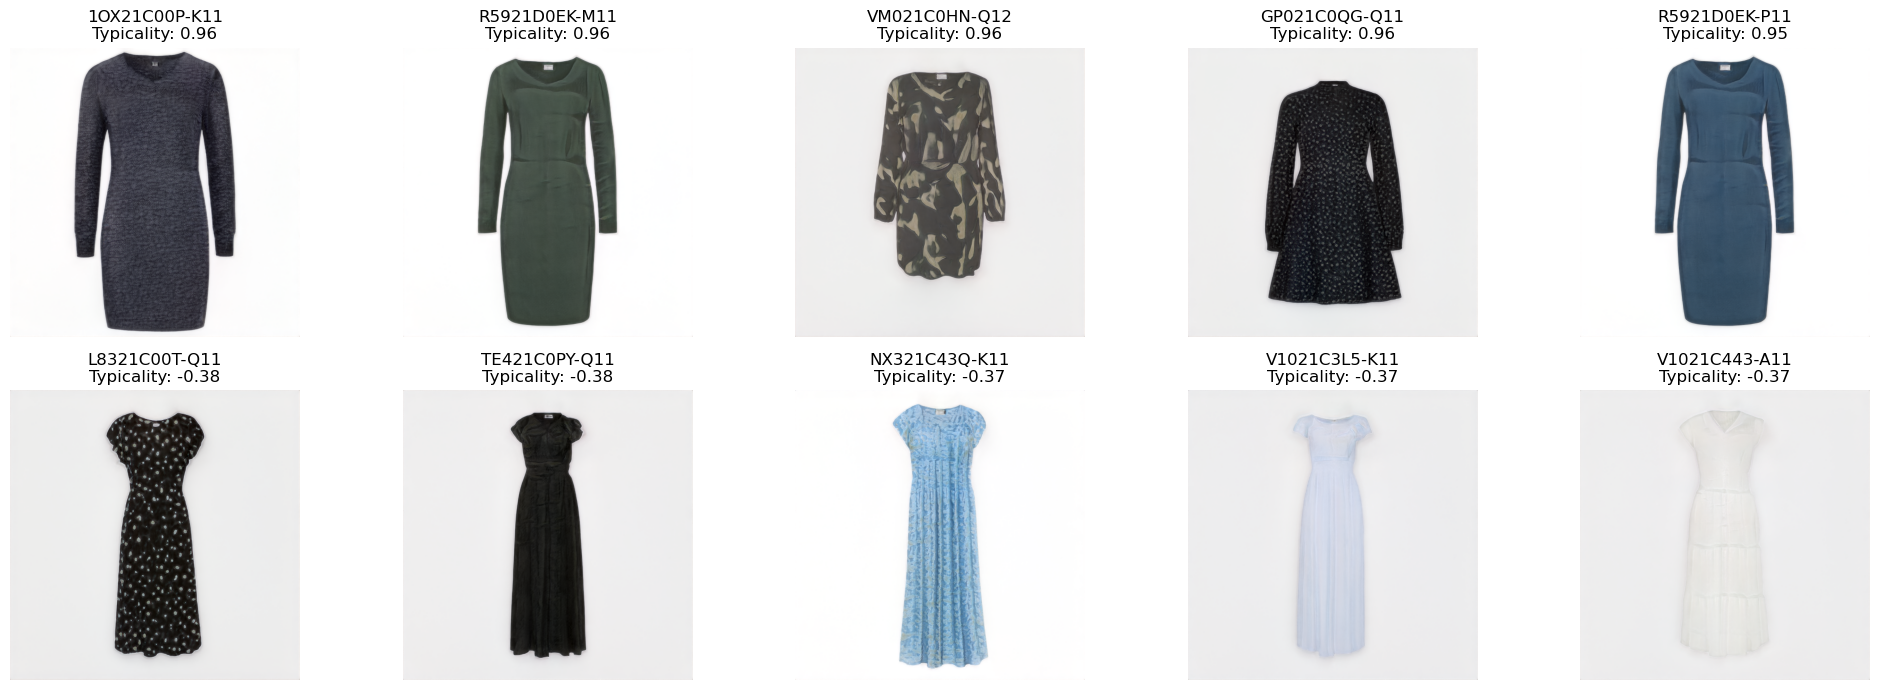
\includegraphics[width=1\linewidth]{Thesis/Results/assets/examples_disentangled_ex_color.png}
    \caption[Most and Least Typical Dresses based on Disentangled Embeddings excluding Color]{Most and Least Typical Dresses based on Disentangled Embeddings excluding Color: \textit{Top row shows samples with the highest typicality scores, bottom row shows samples with the lowest typicality scores}}
    \label{fig:examples_disentangled_ex_color}
\end{figure}

\begin{figure}[!ht]
    \centering
    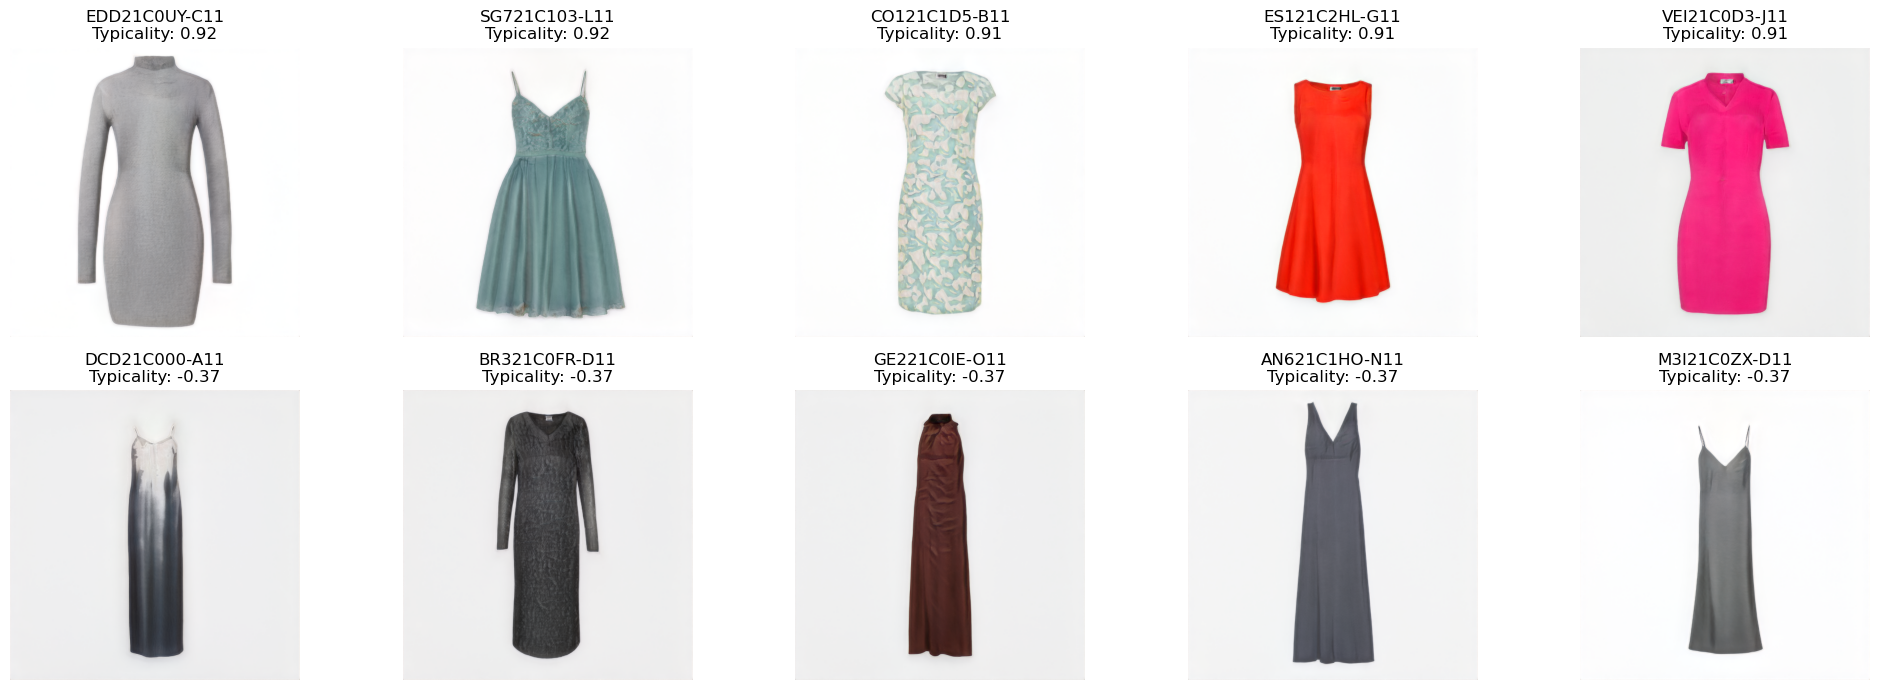
\includegraphics[width=1\linewidth]{Thesis/Results/assets/examples_disentangled_ex_sleevel_length.png}
    \caption[Most and Least Typical Dresses based on Disentangled Embeddings excluding Sleeve Length]{Most and Least Typical Dresses based on Disentangled Embeddings excluding Sleeve Length: \textit{Top row shows samples with the highest typicality scores, bottom row shows samples with the lowest typicality scores}}
    \label{fig:examples_disentangled_ex_sleevel_length}
\end{figure}

\begin{figure}[!ht]
     \centering
     \begin{subfigure}[b]{0.48\textwidth}
         \centering
         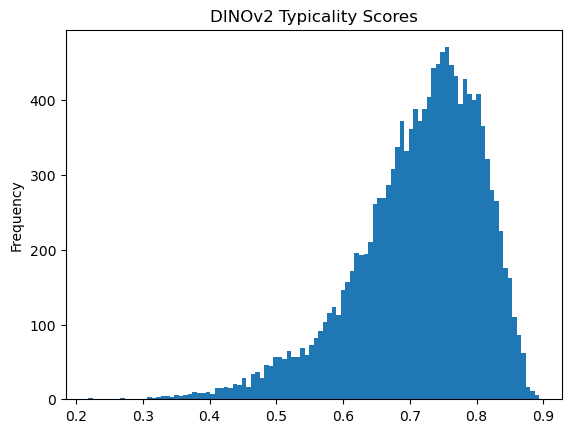
\includegraphics[width=\textwidth]{Thesis/Results/assets/distribution_dino_typicality.png}
         \caption{DINOv2 Embeddings}
     \end{subfigure}
     \hfill
     \begin{subfigure}[b]{0.48\textwidth}
         \centering
         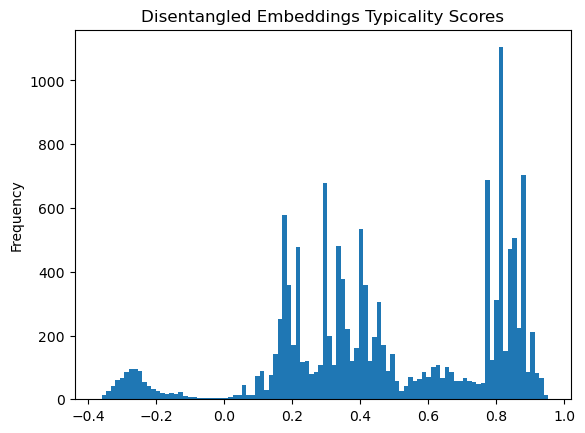
\includegraphics[width=\textwidth]{Thesis/Results/assets/distribution_disentangled_typicality.png}
         \caption{Disentangled Embeddings}
     \end{subfigure}
     \hfill
\caption{Distribution of typicality scores}
\label{fig:typicality_score_distribution}
\end{figure}

\FloatBarrier
\subsection*{Hyperstyle Manipulation Results}
\begin{figure}[!ht]
    \centering
    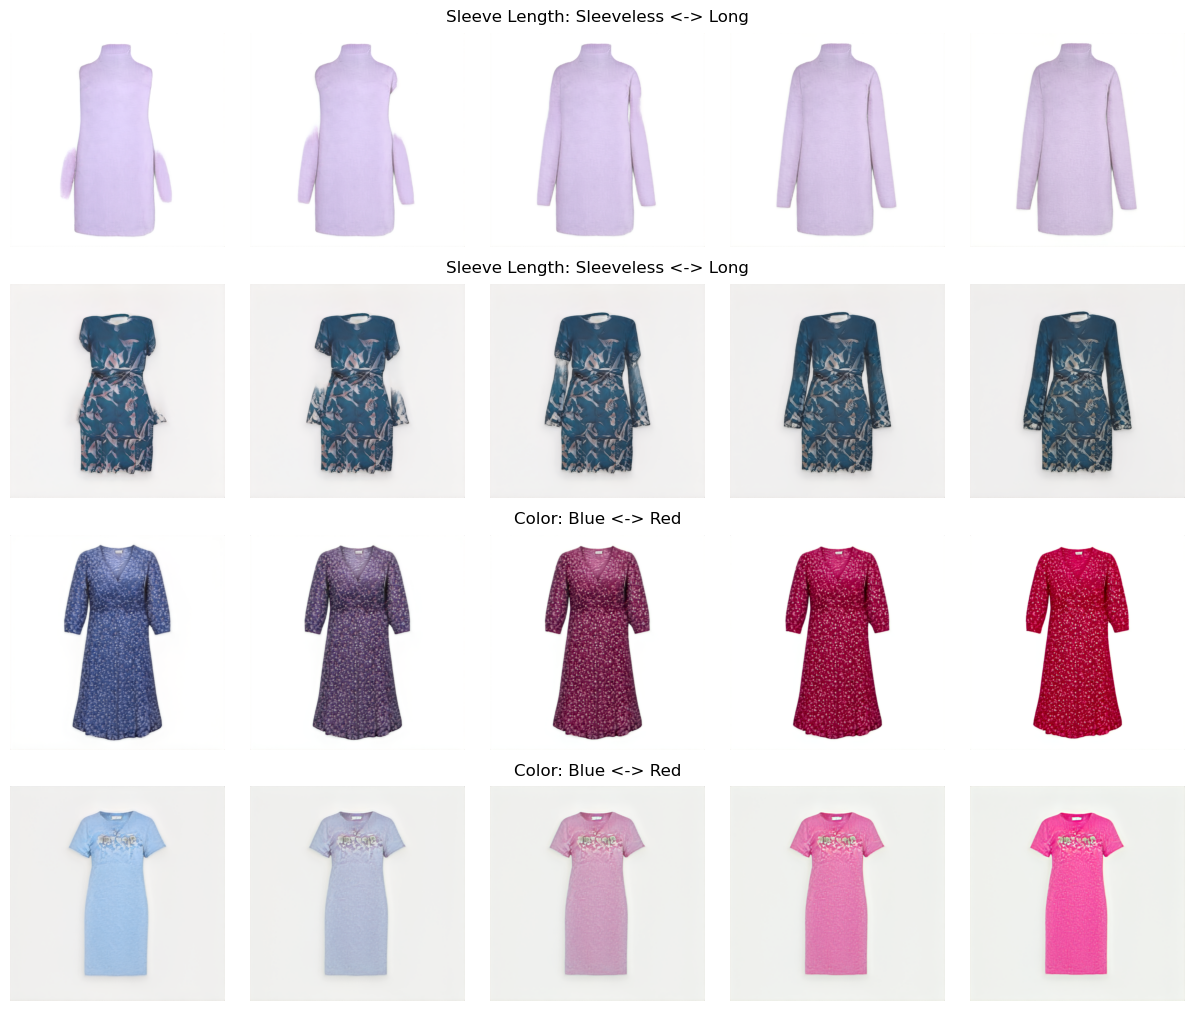
\includegraphics[width=1\linewidth]{Thesis/Results/assets/hyperstyle_manipulation_tests.png}
    \caption[Preliminary Manipulation Tests using Hyperstyle Inversions]{Preliminary Manipulation Tests using Hyperstyle Inversions: \textit{To assess the overall suitability of Hyperstyle Inversions for the InterFaceGAN scheme, manipulation of visual attributes is tested. Although some manipulations seem to work well, others, especially the sleeve length manipulations, produce faulty artifacts.}}
    \label{fig:hyperstyle_manipulation_tests}
\end{figure}


\FloatBarrier
\newpage
\subsection*{Distance Correlation Formulas}
Below, detailed formulas for the calculation of the distance correlation are given. All formulas and explanations are directly taken or slightly adapted from \cite{muller2024disentangling}, p.5.
\begin{equation}\label{eq:dcor_formula}
\text{dCor}(w_1, w_2) = \sqrt{\frac{\text{dCov}^2(w_1, w_2)}{(\text{dVar}^2(w_1) \text{dVar}^2(w_2))^{1/2}}}
\end{equation}

Assuming \(n\)-dimensional batches of subspace vectors \(w_1 \in \mathbb{R}^{n \times d_1}\) and \(w_2 \in \mathbb{R}^{n \times d_2}\), a \(n \times n\) dimensional Euclidean space containing all pairwise distances can be calculated as
\begin{equation}
A \in \mathbb{R}^{n \times n}, \quad a_{j,k} = \|w_1^{(j)} - w_1^{(k)}\|_2, \quad j, k = 1, 2, \dots, n
\end{equation}
\begin{equation}
B \in \mathbb{R}^{n \times n}, \quad b_{j,k} = \|w_2^{(j)} - w_2^{(k)}\|_2, \quad j, k = 1, 2, \dots, n
\end{equation}

Normalization of the distance matrices was performed by subtracting the row mean, column mean, and grand mean. Formally, this can be expressed as
\begin{equation}
A_{j,k} := a_{j,k} - \bar{a}_{j,\cdot} - \bar{a}_{\cdot,k} + \bar{a}_{\cdot,\cdot}
\end{equation}
\begin{equation}
B_{j,k} := b_{j,k} - \bar{b}_{j,\cdot} - \bar{b}_{\cdot,k} + \bar{b}_{\cdot,\cdot}
\end{equation}

Finally, $\text{dCov}^2$ can be calculated as the arithmetic mean of the element-wise matrix product.
\begin{equation}
\text{dCov}^2(w_1, w_2) = \frac{1}{n^2} \sum_{j=1}^{n} \sum_{k=1}^{n} A_{j,k} B_{j,k}
\end{equation}
$\text{dVar}^2$ can be calculated as the arithmetic mean of the squared matrix elements of the normalized distance matrices.
\begin{equation}
\text{dVar}^2(w_1) = \frac{1}{n^2} \sum_{j,k} A_{j,k}^2
\end{equation}
\begin{equation}\label{eq:last_dcor_formula}
\text{dVar}^2(w_2) = \frac{1}{n^2} \sum_{j,k} B_{j,k}^2
\end{equation}

\FloatBarrier

%\subsection*{Unconditional Typicality Manipulation}

\clearpage
\begin{figure}[!ht]
    \centering
    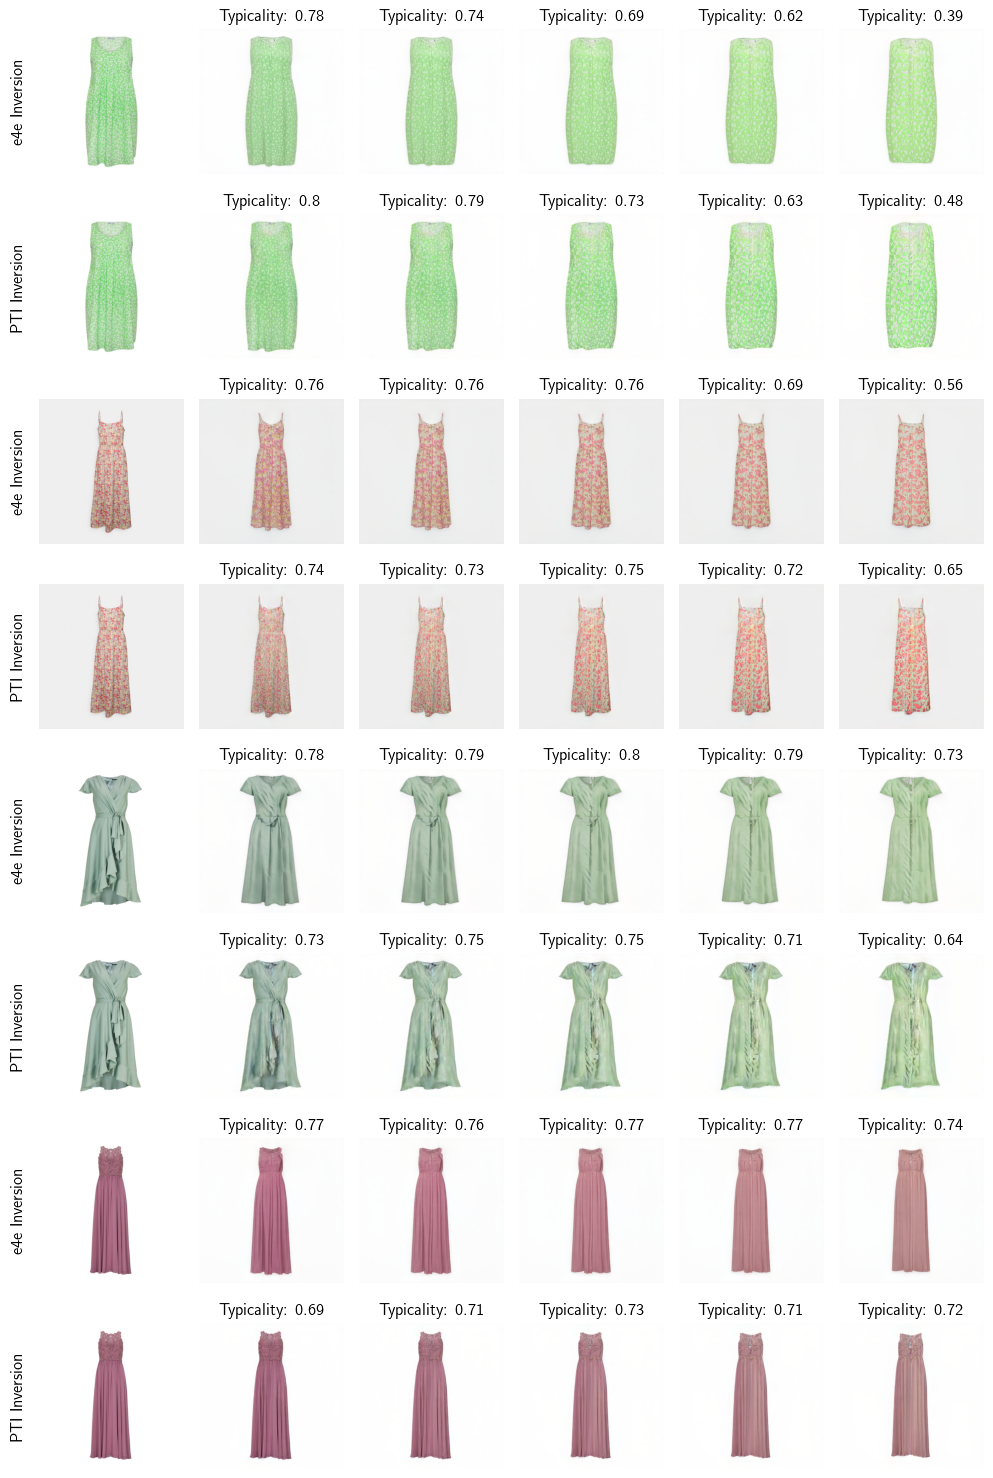
\includegraphics[width=0.9\linewidth]{Thesis/Results/assets/dino_less.png}
    \caption[Decreasing Typicality for DINOv2 Embeddings]{Decreasing Typicality for DINOv2 Embeddings: \textit{First row shows the original image, second row is the inversion. All following rows are each +5 InterFaceGAN steps towards less typicality}}
    \label{fig:dino_less}
\end{figure}

\clearpage
\begin{figure}[!ht]
    \centering
    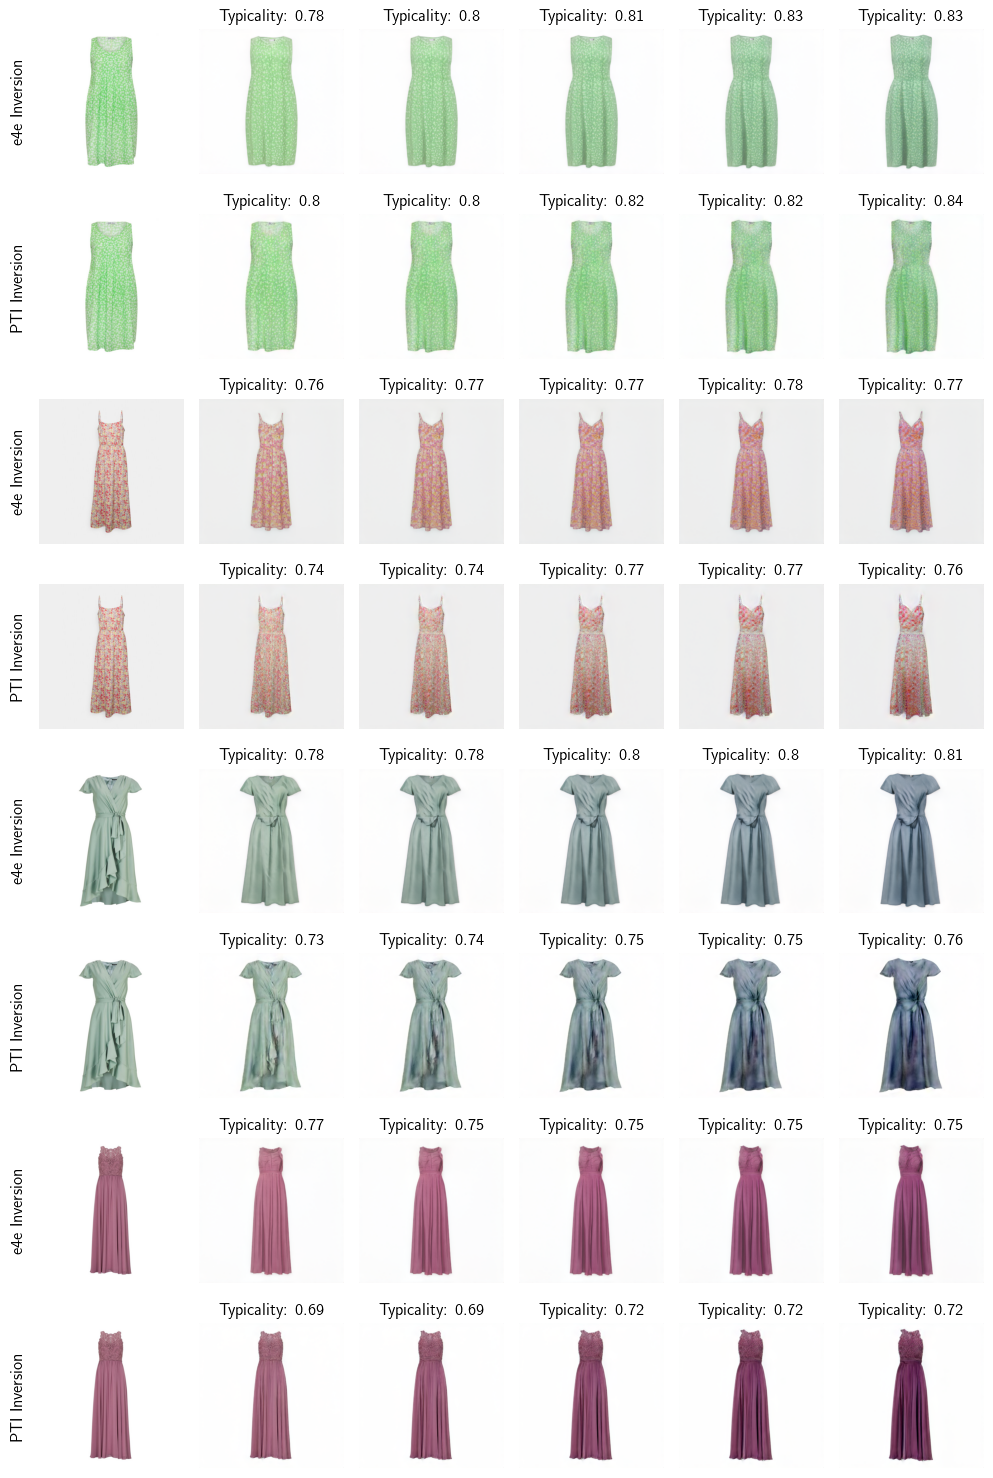
\includegraphics[width=0.9\linewidth]{Thesis/Results/assets/dino_more.png}
    \caption[Increasing Typicality for DINOv2 Embeddings]{Increasing Typicality for DINOv2 Embeddings: \textit{First row shows the original image, second row is the inversion. All following rows are each +5 InterFaceGAN steps towards more typicality}}
    \label{fig:dino_more}
\end{figure}


\clearpage
\begin{figure}[!ht]
    \centering
    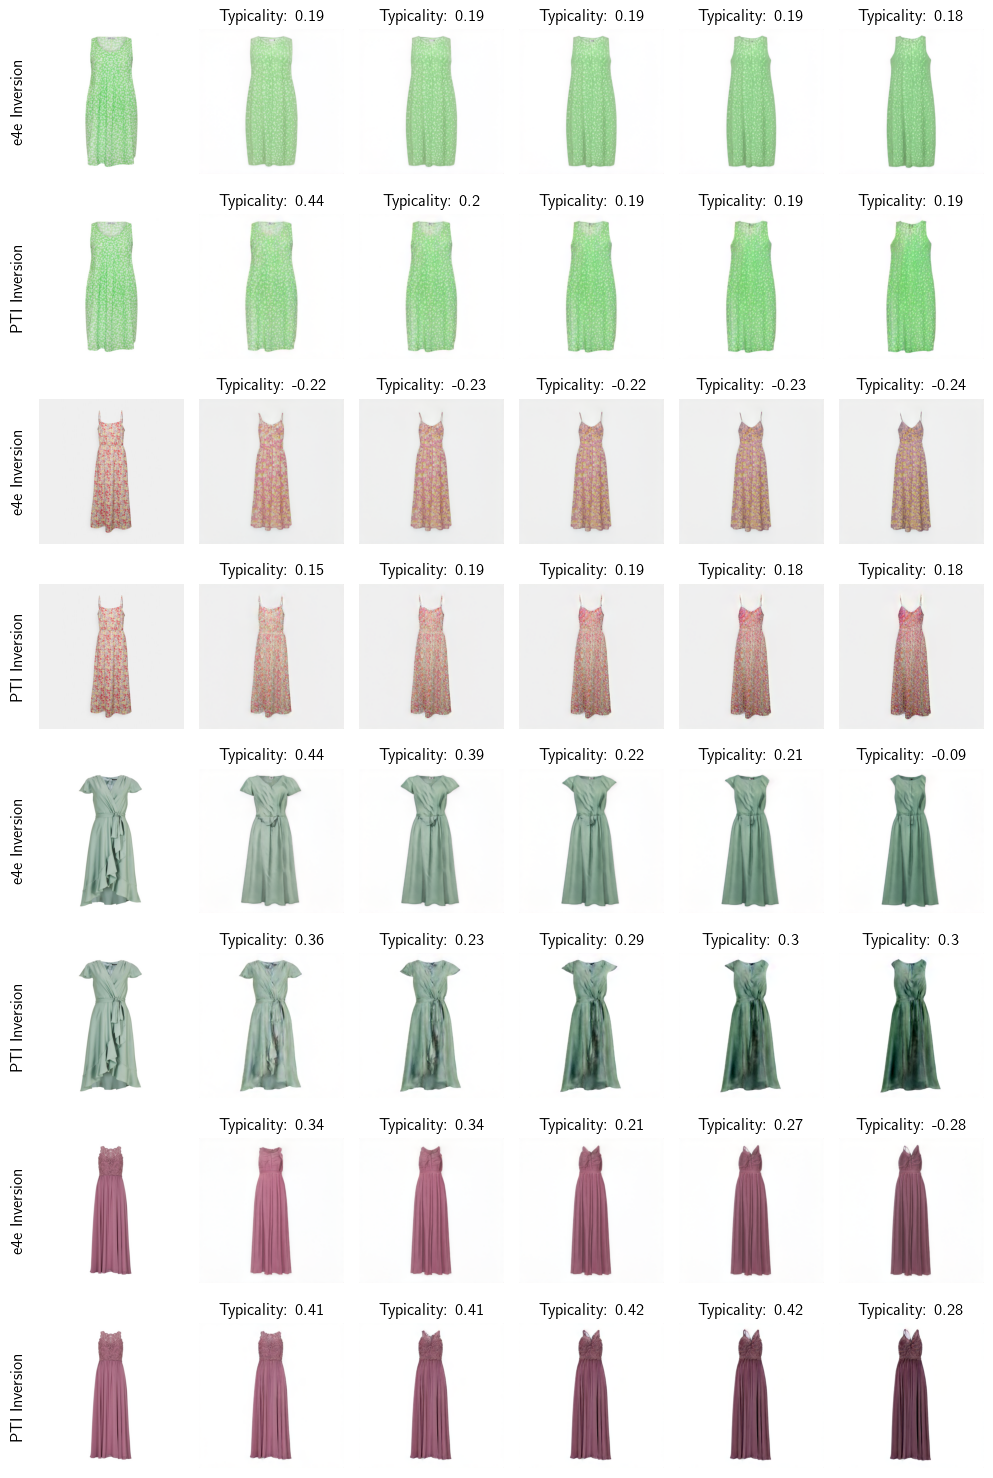
\includegraphics[width=0.9\linewidth]{Thesis/Results/assets/disentangled_less.png}
    \caption[Decreasing Typicality for Disentangled Embeddings]{Decreasing Typicality for Disentangled Embeddings: \textit{First row shows the original image, second row is the inversion. All following rows are each +5 InterFaceGAN steps towards less typicality}}
    \label{fig:disentangled_less}
\end{figure}

\clearpage
\begin{figure}[!ht]
    \centering
    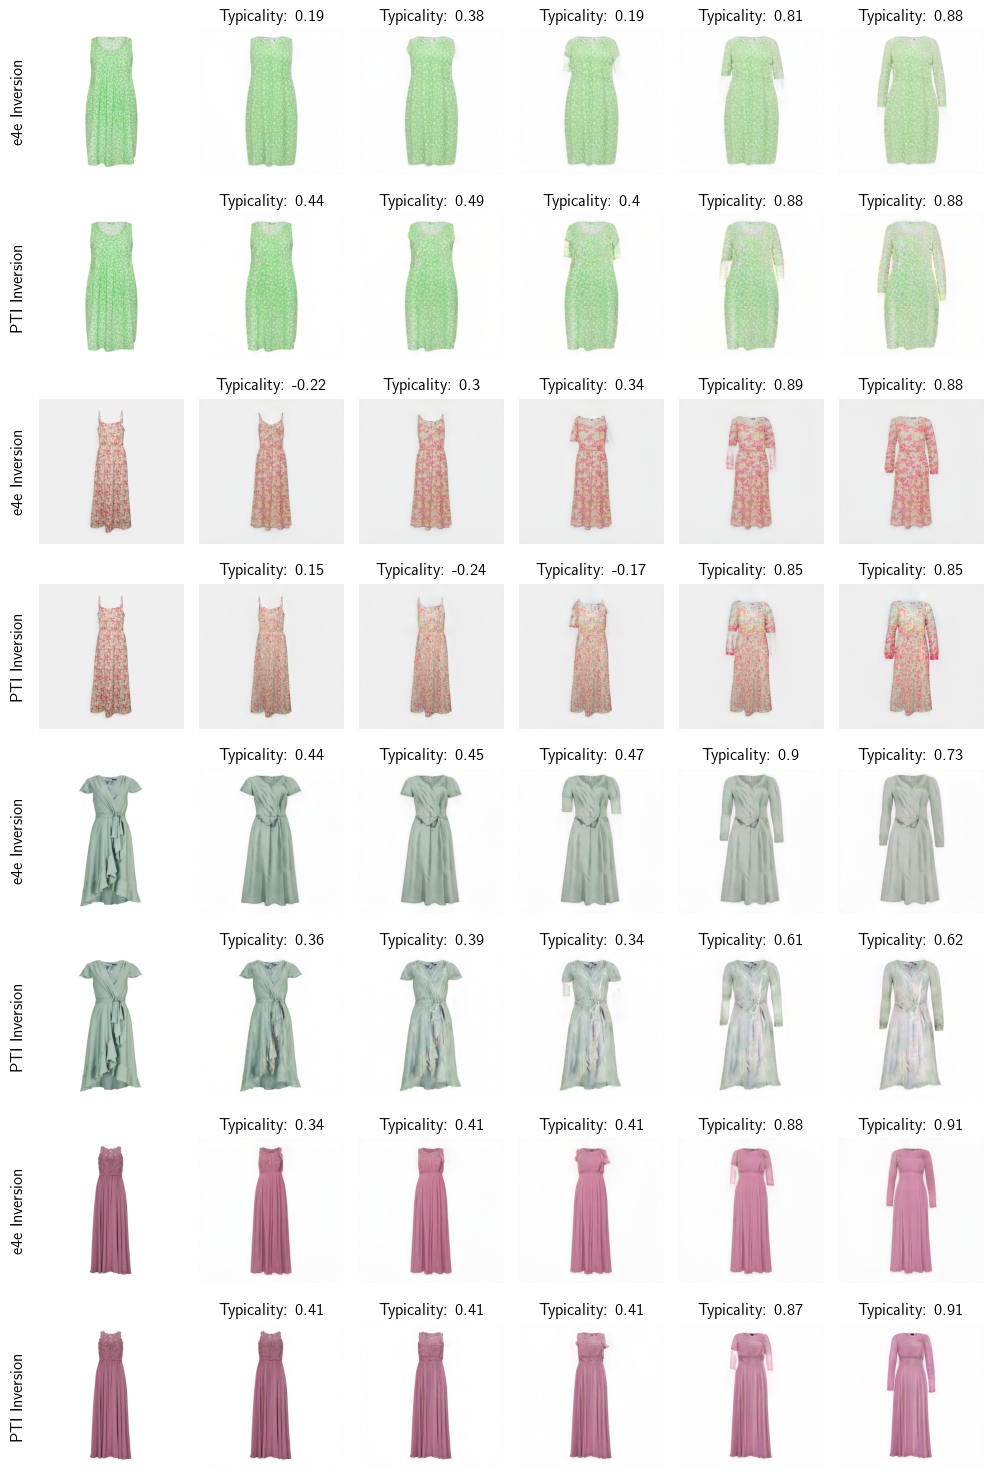
\includegraphics[width=0.9\linewidth]{Thesis/Results/assets/disentangled_more.png}
    \caption[Increasing Typicality for Disentangled Embeddings]{Increasing Typicality for Disentangled Embeddings: \textit{First row shows the original image, second row is the inversion. All following rows are each +5 InterFaceGAN steps towards more typicality}}
    \label{fig:disentangled_more}
\end{figure}

\clearpage
\begin{figure}[!ht]
    \centering
    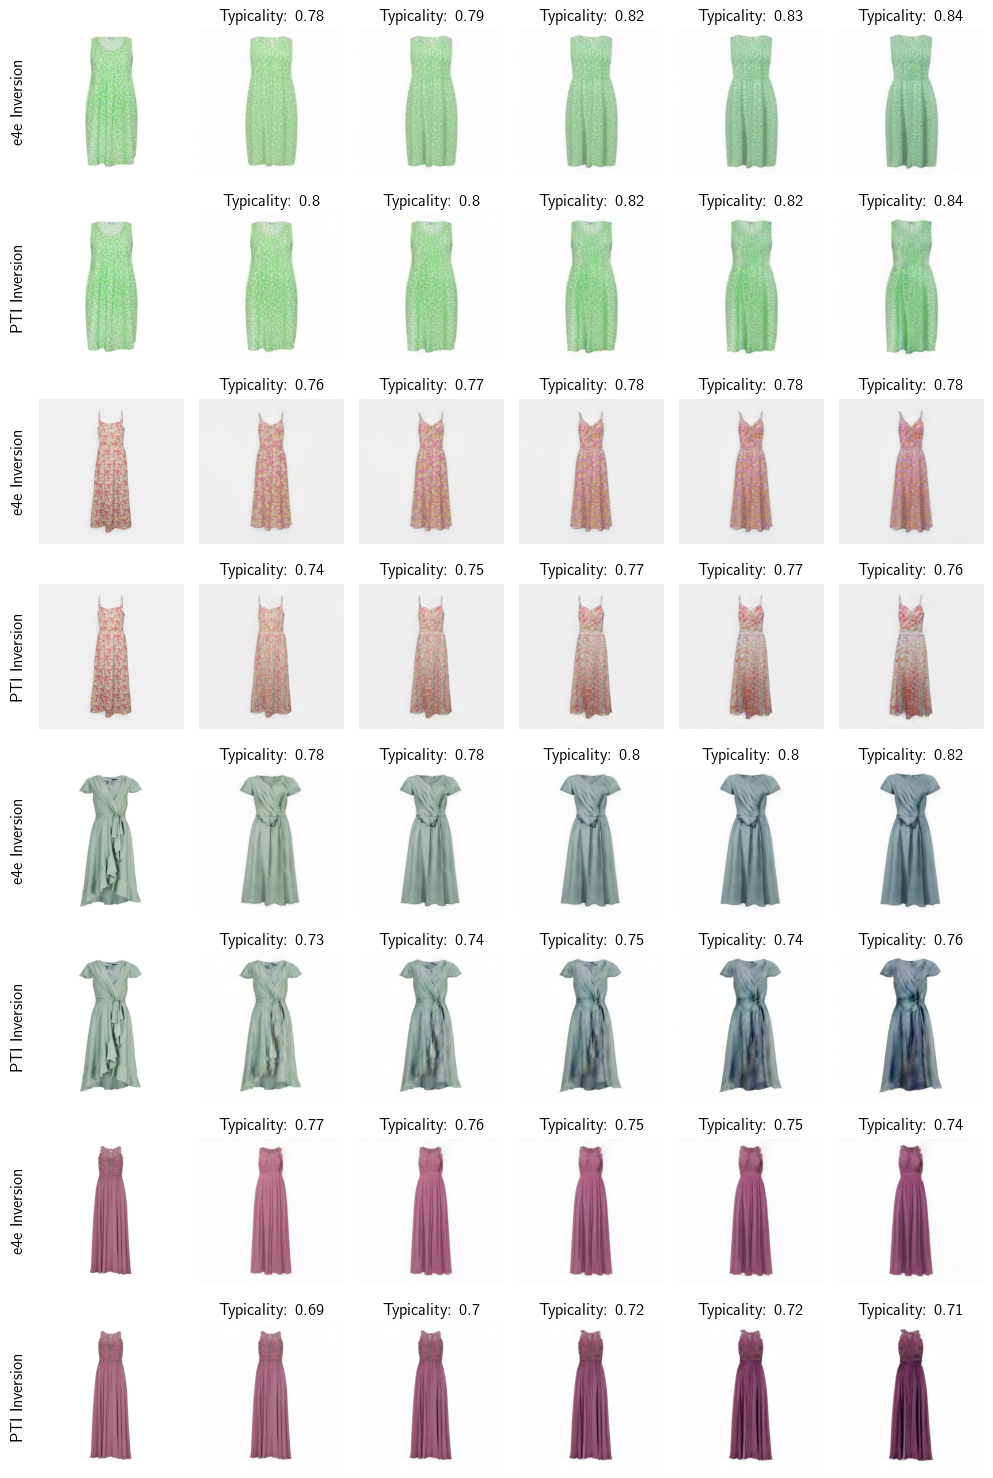
\includegraphics[width=0.9\linewidth]{Thesis/Results/assets/dino_cond_color_more.png}
    \caption[Increasing Typicality for DINOv2 Embeddings conditioned on Color]{Increasing Typicality for DINOv2 Embeddings conditioned on Color: \textit{First row shows the original image, second row is the inversion. All following rows are each +5 InterFaceGAN steps towards more typicality}}
    \label{fig:dino_cond_color_more}
\end{figure}

\clearpage
\begin{figure}[!ht]
    \centering
    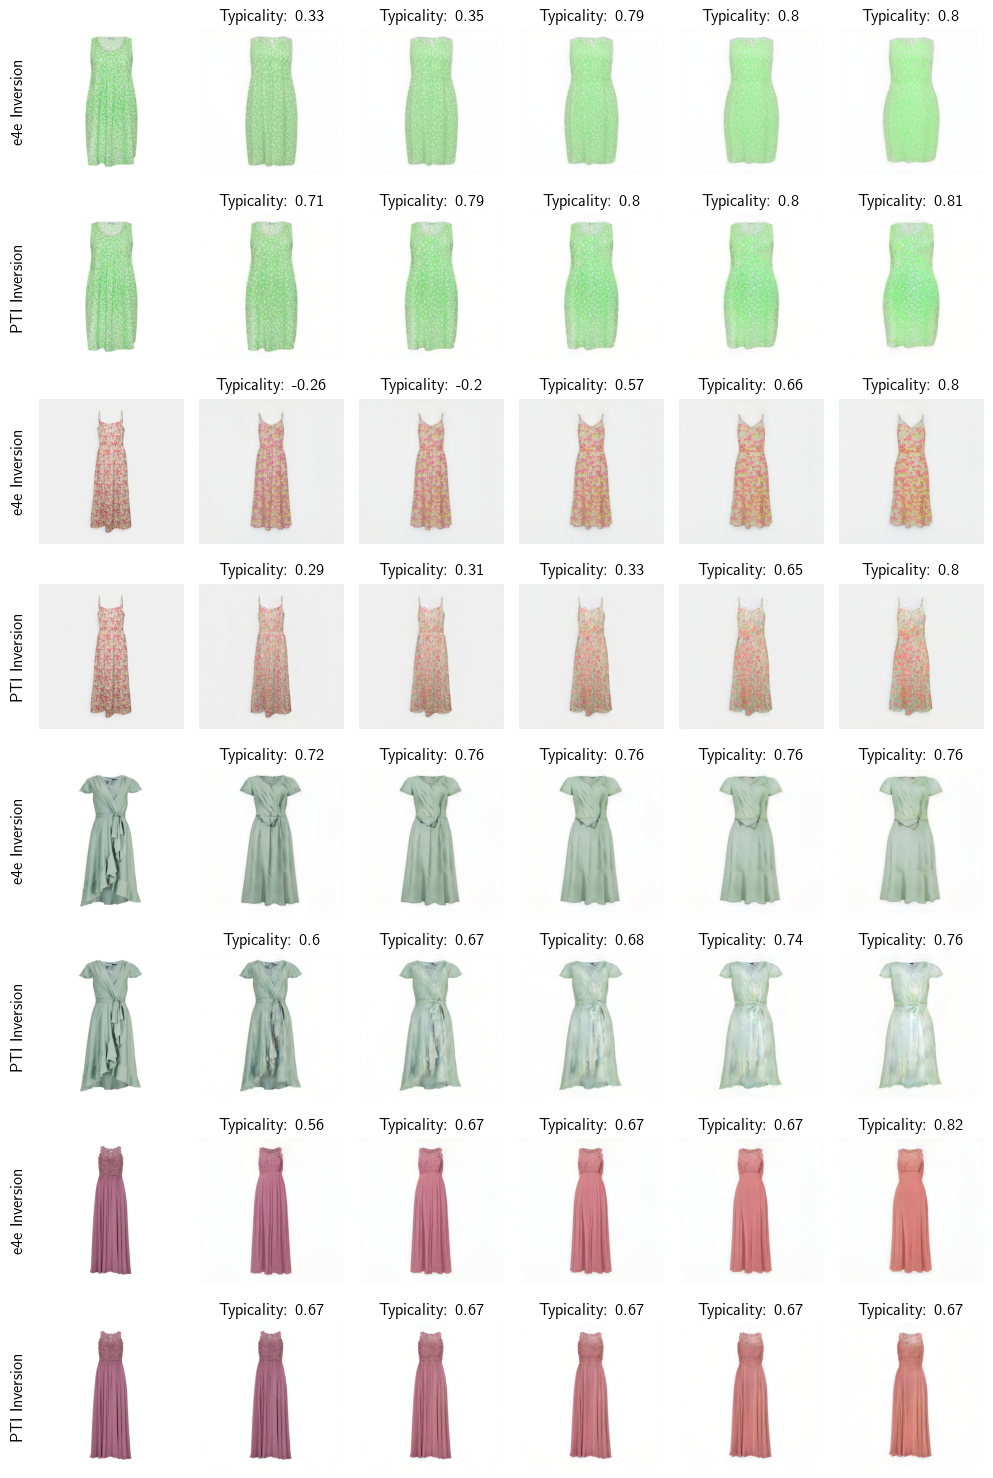
\includegraphics[width=0.9\linewidth]{Thesis/Results/assets/disentangled_ex_sleeve_more.png}
    \caption[Increasing Typicality for Disentangled Embeddings excl. Sleeve Length]{Increasing Typicality for Disentangled Embeddings excl. Sleeve Length: \textit{First row shows the original image, second row is the inversion. All following rows are each +5 InterFaceGAN steps towards more typicality}}
    \label{fig:disentangled_ex_sleeve_more}
\end{figure}

\clearpage
\begin{figure}[!ht]
    \centering
    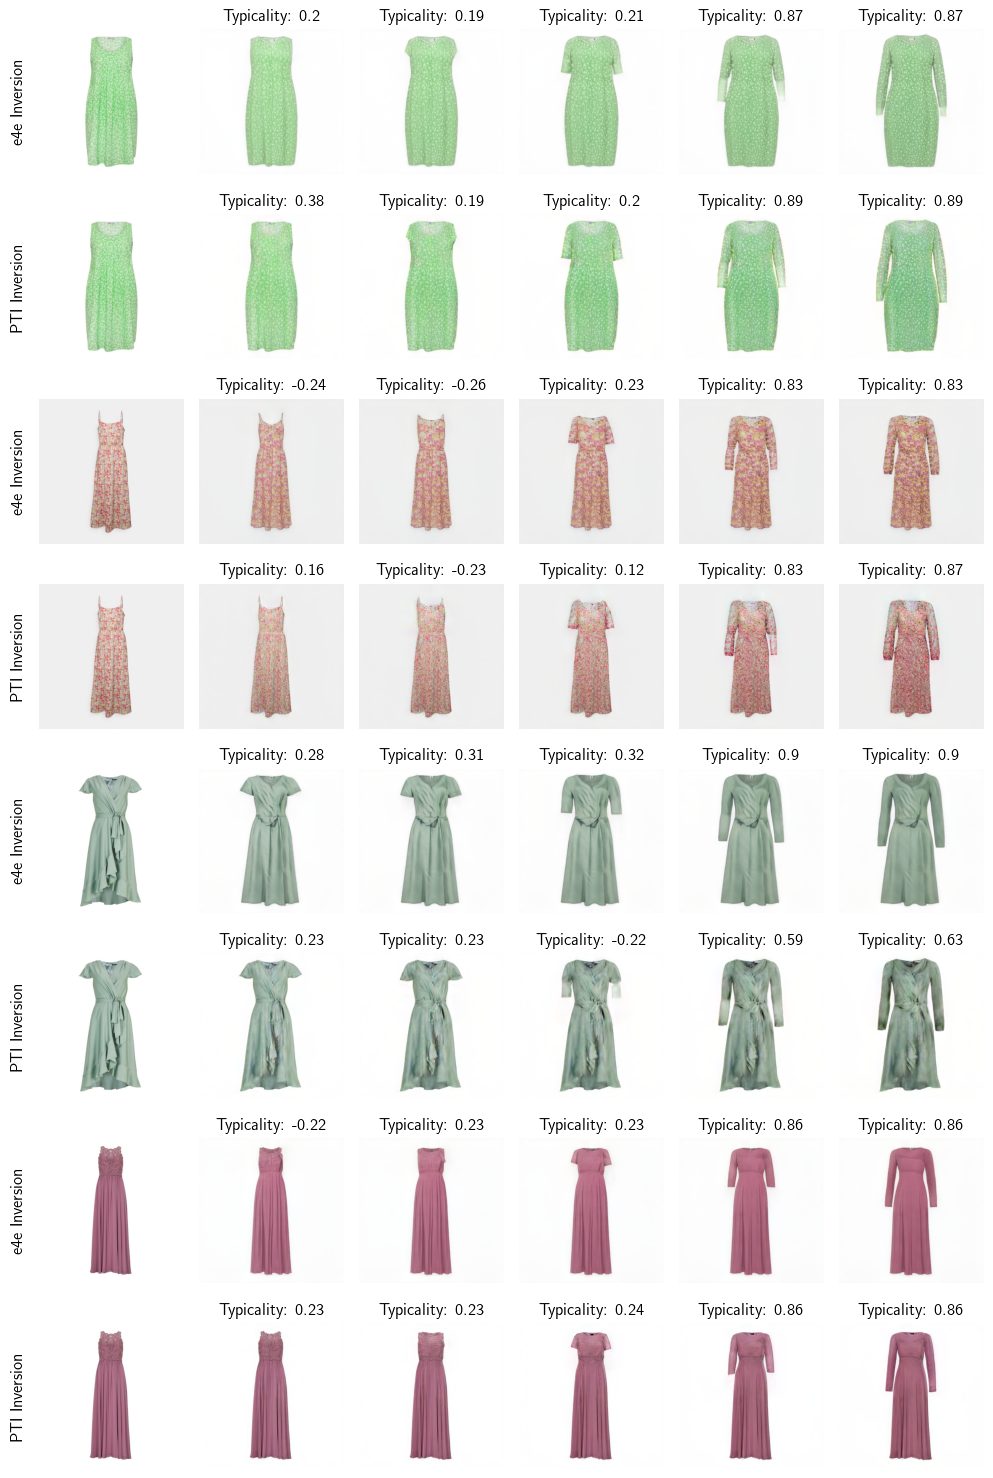
\includegraphics[width=0.9\linewidth]{Thesis/Results/assets/disentangled_ex_color_more.png}
    \caption[Increasing Typicality for Disentangled Embeddings excl. Color]{Increasing Typicality for Disentangled Embeddings excl. Color: \textit{First row shows the original image, second row is the inversion. All following rows are each +5 InterFaceGAN steps towards more typicality}}
    \label{fig:disentangled_ex_color_more}
\end{figure}



